% =====================================================================
% 20-minute presentation — Acemoglu & Restrepo (NBER WP 22252, June 2017)
% Repository ai-06-restrepo. No animations, no screenshots of the paper;
% every equation is typeset. Compile: latexmk -pdf presentation.tex
% =====================================================================
\documentclass[aspectratio=169,10pt]{beamer}
\usetheme[progressbar=frametitle,numbering=fraction]{metropolis}
\usepackage[T1]{fontenc}
\usepackage[utf8]{inputenc}
\IfFileExists{spanish.ldf}{\usepackage[spanish,es-noshorthands,es-nodecimaldot]{babel}}{}
\usepackage{amsmath,amssymb,mathtools,booktabs,array}
\usepackage{tikz,pgfplots,listings,xcolor}
\pgfplotsset{compat=1.17}
\usetikzlibrary{decorations.pathreplacing,arrows.meta}

% ---------- EDIT HERE: your GitHub user ----------
\newcommand{\repourl}{https://github.com/alejandroventuraventurameza-tech/ai-06-restrepo}

\newcommand{\sh}{\hat\sigma}
\newcommand{\It}{\tilde I}
\newcommand{\Is}{I^{*}}
\newcommand{\Kl}{\underline K}
\newcommand{\Kb}{\overline K}
\newcommand{\Kh}{\hat K}
\newcommand{\eps}{\varepsilon}
\definecolor{posc}{HTML}{1B7F3B}
\definecolor{negc}{HTML}{B3261E}
\definecolor{leanbg}{HTML}{F5F5F2}

% ---------- Lean listings (unicode mapped to math) ----------
\lstdefinelanguage{lean}{
  morekeywords={theorem,lemma,def,by,have,exact,fun,rintro,set,with,show,intro,rw,refine,obtain,absurd,Prop},
  sensitive=true, morecomment=[l]{--}, morestring=[b]"}
\lstset{language=lean, basicstyle=\ttfamily\scriptsize, keywordstyle=\color{blue!60!black}\bfseries,
  commentstyle=\color{gray}\itshape, backgroundcolor=\color{leanbg}, frame=single, rulecolor=\color{gray!40},
  columns=fullflexible, keepspaces=true, breaklines=true, xleftmargin=2pt, xrightmargin=2pt,
  escapeinside={(*}{*)}}

\title{La carrera entre la máquina y el hombre}
\subtitle{Acemoglu \& Restrepo (NBER WP 22252, jun.\ 2017)}
\author{Alejandro Ventura}
\institute{IA y Modelamiento Económico — UP 2026-II\quad\textbullet\quad Repositorio: \url{\repourl}}
\date{25 de septiembre de 2026}

\begin{document}
\maketitle

% =====================================================================
\section{El paper y el problema}
% =====================================================================

\begin{frame}{La pregunta, la respuesta y el aporte}
\small
\begin{columns}[T]
\column{0.52\textwidth}
\textbf{Pregunta} (no el tema): ¿puede una economía crecer de forma balanceada mientras el capital reemplaza
tareas del trabajo, \emph{sin} volver redundante al trabajo? ¿Qué fuerzas de mercado hacen que la automatización se autolimite?

\medskip
\textbf{Respuesta}, en tres capas:
\begin{enumerate}\setlength\itemsep{2pt}
  \item \emph{Estática}: la automatización baja la participación laboral y el empleo, y \emph{puede} bajar el salario.
  \item \emph{Capital endógeno}: a largo plazo el salario sube; la participación sigue bajando.
  \item \emph{Tecnología endógena}: la senda con tareas nuevas y automatización a la par es estable, salvo que el capital sea muy barato.
\end{enumerate}
\column{0.45\textwidth}
\textbf{Aporte frente a predecesores}
\begin{itemize}\setlength\itemsep{2pt}
  \item \textbf{Zeira (1998)}: solo automatiza; es un caso particular. Sin tareas nuevas, $s_L\to0$.
  \item \textbf{Acemoglu--Autor (2011)}: tareas, pero estático y exógeno.
  \item \textbf{Acemoglu (2002, 2003)}: cambio dirigido que \emph{aumenta factores}; la estabilidad exige elasticidad $<1$. Aquí no.
\end{itemize}
\end{columns}
\end{frame}

\begin{frame}{Un cambio de unidad de análisis: la economía agregada}
\small
\begin{columns}[c]
\column{0.5\textwidth}
En los cinco papers anteriores del curso había \emph{un agente} que decidía (esfuerzo, adopción de IA\ldots).

\medskip
Aquí nadie resuelve un problema interesante por sí solo:
\begin{itemize}
  \item cada firma minimiza el costo de \emph{una} tarea;
  \item el hogar ofrece trabajo: $L=L^s(W/RK)$.
\end{itemize}
El objeto de estudio es la \textbf{asignación de tareas a factores} en toda la economía, y cómo esa asignación fija precios y participaciones.
\column{0.46\textwidth}
\begin{block}{``El problema del agente'', reescrito}
\[
  p(i)=\begin{cases}\min\{R,\ W/\gamma(i)\} & i\le I\\ W/\gamma(i) & i>I\end{cases}
\]
\[
  \Is=\min\{I,\It\},\qquad \frac WR=\gamma(\It)
\]
Un punto fijo: el umbral depende de precios que dependen del umbral.
\end{block}
\end{columns}
\end{frame}

\begin{frame}{El marco de tareas}
\centering
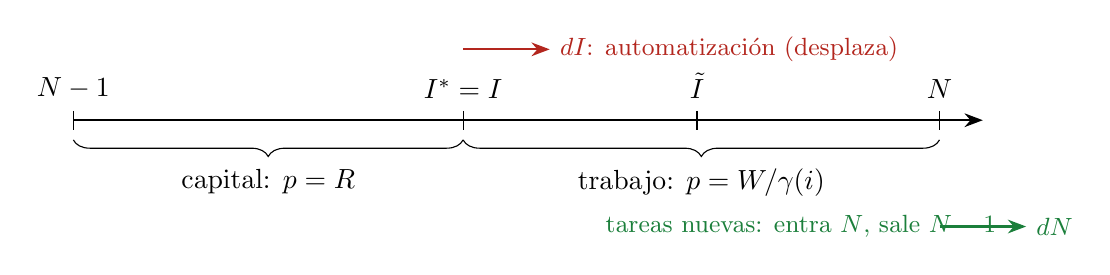
\begin{tikzpicture}[x=11cm,y=1cm,>=Stealth]
  \draw[thick,->] (0,0) -- (1.05,0);
  \foreach \x/\l in {0/{N-1},0.45/{\Is=I},0.72/{\It},1/{N}} {\draw (\x,0.12)--(\x,-0.12); \node[above] at (\x,0.15) {$\l$};}
  \draw[decorate,decoration={brace,mirror,amplitude=6pt}] (0,-0.25) -- (0.45,-0.25) node[midway,below=7pt] {capital: $p=R$};
  \draw[decorate,decoration={brace,mirror,amplitude=6pt}] (0.45,-0.25) -- (1,-0.25) node[midway,below=7pt] {trabajo: $p=W/\gamma(i)$};
  \draw[->,negc,thick] (0.45,0.9) -- (0.55,0.9) node[right,font=\small] {$dI$: automatización (desplaza)};
  \draw[->,posc,thick] (1,-1.35) -- (1.1,-1.35) node[right,font=\small] {$dN$};
  \node[posc,font=\small,align=left] at (0.84,-1.35) {tareas nuevas: entra $N$, sale $N-1$};
\end{tikzpicture}

\vspace{6pt}
\begin{itemize}\small
  \item Continuo de tareas de medida 1, agregado con una CES: $Y=\tilde B\big(\int_{N-1}^N y(i)^{\frac{\sigma-1}{\sigma}}di\big)^{\frac{\sigma}{\sigma-1}}$.
  \item \textbf{Supuesto 1}: $\gamma$ estrictamente creciente (el trabajo tiene ventaja comparativa en tareas complejas), lo que genera un umbral.
  \item \textbf{Supuesto 2}: $\eta\to0$ o $\zeta=1$ (homotecia). \textbf{Supuesto 3}: $R>W/\gamma(N)$ (las tareas nuevas se usan).
\end{itemize}
\end{frame}

\begin{frame}{Equilibrio: tres regímenes, no dos}
\begin{columns}[T]
\column{0.5\textwidth}
\textbf{Prop.~1}: existe un único equilibrio y el producto es una CES con \emph{pesos endógenos}:
\[
Y=\tfrac{B}{1-\eta}\Big[a^{\frac1\sh}K^{\frac{\sh-1}{\sh}}+\Gamma^{\frac1\sh}L^{\frac{\sh-1}{\sh}}\Big]^{\frac{\sh}{\sh-1}}
\]
con $a=\Is-N+1$ y $\Gamma=\int_{\Is}^N\gamma^{\sh-1}$.

\medskip
Automatizar cambia la \emph{función de producción}, no la eficiencia de un factor.
\column{0.47\textwidth}
\small
\begin{tabular}{@{}lll@{}}
\toprule
Régimen & Condición & Efecto de $I$\\
\midrule
(R) restringido & $\Is=I<\It$ & activo\\
(L) libre & $\Is=\It<I$ & nulo\\
(F) frontera & $\Is=I=\It$ & excluido\\
\bottomrule
\end{tabular}

\medskip
En (R) las firmas querrían automatizar más: $W/\gamma(I)>R$. En (F) las derivadas laterales difieren; el paper lo omite (nota 15).
\end{columns}
\end{frame}

% =====================================================================
\section{El resultado principal, con todas sus condiciones}
% =====================================================================

\begin{frame}{Prop.~2: la automatización siempre sesga contra el trabajo}
De $\ \sh\ln\omega+\ln L^s(\omega)=\ln\Gamma(\Is)-\ln a(\Is)+(1-\sh)\ln K$, con $\omega=W/(RK)$:
\[
\frac{d\ln\omega}{dI}=-\frac{\Lambda_I}{\sh+\eps_L}<0,\qquad
\Lambda_I=\frac{\gamma(I)^{\sh-1}}{\int_I^N\gamma^{\sh-1}}+\frac{1}{I-N+1}>0,
\qquad \frac{d\ln\omega}{dN}=\frac{\Lambda_N}{\sh+\eps_L}>0.
\]
\begin{itemize}
  \item La participación laboral $s_L$ y el empleo se mueven con $\omega$, así que en (R) \textbf{siempre caen} con $I$, para \emph{cualquier} $\sh$.
  \item Contraste: con tecnología que aumenta factores, el sesgo depende de si $\sh\gtrless1$.
  \item En (L), $\sigma^{\text{free}}=\sh+\Lambda_I/\eps_\gamma>\sh$: el umbral también se ajusta.
  \item Condiciones: Supuestos 1–3, $\eps_L>0$; sin el Supuesto 2, hace falta el 2$'$ (no homotecia acotada).
\end{itemize}
\end{frame}

\begin{frame}{Prop.~3: dos fuerzas con signo opuesto}
\[
\frac{d\ln W}{dI}=
\underbrace{B^{\sh-1}\!\int_{R}^{W/\gamma(I)}\!x^{-\sh}\,dx}_{\textcolor{posc}{\text{productividad }(+)}}
\;-\;
\underbrace{(1-s_L)\frac{\Lambda_I}{\sh+\eps_L}}_{\textcolor{negc}{\text{desplazamiento }(-)}}
\qquad\text{(caso R)}
\]
\small
\begin{columns}[T]
\column{0.55\textwidth}
\begin{tabular}{@{}llccc@{}}
\toprule
 & fuerza & $W$ & $R$ & $s_L,L$\\
\midrule
$dI$ & productividad & $+$ & $+$ & 0\\
 & desplazamiento & $-$ & $+$ & $-$\\
\midrule
$dN$ & productividad & $+$ & $+$ & 0\\
 & reinstauración & $+$ & $-$ & $+$\\
\bottomrule
\end{tabular}
\column{0.42\textwidth}
\begin{itemize}\setlength\itemsep{2pt}
  \item El paper escribe $\frac{B^{\sh-1}}{1-\sh}[(W/\gamma)^{1-\sh}-R^{1-\sh}]$, que no está definido en $\sh=1$. La integral cubre todos los casos.
  \item ``Reinstauración'' no aparece en la versión 2017: es el término de $dN$ (AR 2019).
\end{itemize}
\end{columns}
\end{frame}

\begin{frame}{La trampa: ¿la automatización baja necesariamente salarios y participación?}
\centering\small
\begin{tabular}{@{}p{2.6cm}>{\centering\arraybackslash}p{4.6cm}>{\centering\arraybackslash}p{2.4cm}>{\centering\arraybackslash}p{3.2cm}@{}}
\toprule
 & corto plazo, (R) & corto plazo, (L) & largo plazo (Prop.~5)\\
\midrule
salario $W$ & \textbf{sube si y solo si} productividad $>$ desplazamiento & $=$ & \textcolor{posc}{sube}\\
participación $s_L$ & \textcolor{negc}{baja} & $=$ & \textcolor{negc}{baja}\\
empleo $L$ & \textcolor{negc}{baja} & $=$ & \textcolor{negc}{baja}\\
producto, $R$ & \textcolor{posc}{suben} & $=$ & $R\to\rho+\delta+\theta g$\\
\bottomrule
\end{tabular}

\vspace{8pt}
\begin{alertblock}{La condición bajo la cual la automatización sube el salario}
\[
B^{\sh-1}\!\int_{R}^{W/\gamma(I)}\!x^{-\sh}\,dx\;>\;(1-s_L)\frac{\Lambda_I}{\sh+\eps_L}
\]
El ahorro de costos en la tarea marginal debe superar el amontonamiento del trabajo en menos tareas.
Las tecnologías ``más o menos'' ($W/\gamma(I)\approx R$) son las que bajan el salario.
\end{alertblock}
\end{frame}

% =====================================================================
\section{Lo que hice: análisis y cómputo}
% =====================================================================

\begin{frame}{Un caso especial que se deriva a mano}
\textbf{Supuestos con nombre}: A1 ($\gamma\uparrow$), A3, LS ($L^s\uparrow$, $\eps_L>0$), C ($\gamma$ continua),
S-$\eta$ ($\eta=0$), S-$\sigma$ ($\sigma=1$, el Corolario~1 del propio paper).

\medskip
Con $a=I-N+1$, $b=N-I$: $\ \ln Y=a\ln\frac Ka+b\ln\frac Lb+\int_I^N\ln\gamma$, $\ W=\frac{bY}{L}$, $\ R=\frac{aY}{K}$, $\ s_L=b$, $\ \omega L^s(\omega)=\frac ba$.

\begin{block}{Teorema 3.3 (derivation/)}
\[
\frac{d\ln W}{dI}=\underbrace{\ln\frac{W}{\gamma(I)R}}_{\textcolor{posc}{+}}-\underbrace{\frac{1}{b\,(1+\eps_L)}}_{\textcolor{negc}{-}},
\qquad \frac{ds_L}{dI}=-1,\qquad \frac{d\ln L}{dI}=-\frac{\eps_L}{1+\eps_L}\frac{1}{ab}<0 .
\]
\end{block}
Coincide exactamente con la Prop.~3 evaluada en $\sh=1$, $\eta=0$ (verificado simbólicamente).
Además, el empleo no depende de $K$: $\omega=\omega^*(b/a)$.
\end{frame}

\begin{frame}{El umbral de capital va al revés de lo impreso}
\begin{columns}[T]
\column{0.5\textwidth}
\textbf{Impreso (p.~13):} existe $\Kb>\Kl$ tal que automatizar \textcolor{posc}{sube} $W$ si $K<\Kb$ y lo \textcolor{negc}{baja} si $K>\Kb$.

\medskip
\textbf{Problemas}
\begin{enumerate}
  \item El Supuesto~3 impone $K<\Kl<\Kb$: la segunda mitad es vacía.
  \item Cerca del borde $K_I$ (donde $W/R=\gamma(I)$), la productividad tiende a 0 y el desplazamiento no, así que $W$ \textcolor{negc}{baja}.
\end{enumerate}
\column{0.47\textwidth}
\begin{block}{Teorema 4.2 (correcto)}
\[
\frac{d\ln W}{dI}>0\iff K>\Kh=K_I\,e^{\frac{1}{b(1+\eps_L)}}
\]
\small
\begin{tabular}{@{}ll@{}}
$K<K_I$ & (L): efecto nulo\\
$K_I<K<\Kh$ & \textcolor{negc}{baja} $W$ (nunca vacía)\\
$\Kh<K<\Kl$ & \textcolor{posc}{sube} $W$ ($\iff \ln\frac{\gamma(N)}{\gamma(I)}>\frac{1}{b(1+\eps_L)}$)\\
\end{tabular}
\end{block}
\textbf{Corolario 4.3}: la frase impresa es falsa para todo $\Kb$.
\end{columns}
\end{frame}

\begin{frame}{La misma dirección con $\sh\neq1$}
\centering
\begin{tikzpicture}
\begin{axis}[width=0.78\textwidth,height=0.52\textheight,xmode=log,log basis x=10,
  xlabel={$K/K_I$ (capital relativo al borde del régimen R)},ylabel={$d\ln W/dI$},
  grid=major,grid style={gray!20},legend pos=south east,legend style={font=\small},
  xmin=1,ymin=-3.6,ymax=1.8]
  \addplot[very thick,blue!70!black] table[x=K_over_KI,y=dlnW_dI,col sep=comma,
     restrict expr to domain={\thisrow{sigma}}{0.4:0.6}] {sim/results/wage_response_curves.csv};
  \addplot[very thick,black] table[x=K_over_KI,y=dlnW_dI,col sep=comma,
     restrict expr to domain={\thisrow{sigma}}{0.9:1.1}] {sim/results/wage_response_curves.csv};
  \addplot[very thick,orange!80!black] table[x=K_over_KI,y=dlnW_dI,col sep=comma,
     restrict expr to domain={\thisrow{sigma}}{1.9:2.1}] {sim/results/wage_response_curves.csv};
  \addplot[dashed,gray] coordinates {(1,0) (70,0)};
  \legend{$\sh=0.5$, $\sh=1$ (fórmula cerrada), $\sh=2$}
\end{axis}
\end{tikzpicture}

\small Equilibrios recalculados desde cero y derivadas por diferencias finitas. $N=1$, $I=0.5$, $\gamma(i)=e^{5i}$, $L^s=\omega^{0.5}$.
Las curvas terminan donde se viola el Supuesto~3.
\end{frame}

\begin{frame}{Verificación computacional (sim/)}
\begin{columns}[T]
\column{0.5\textwidth}
\textbf{Simbólica (SymPy, sin números): 17/17}
\begin{itemize}\small
  \item re-deriva los Lemas 3.1–3.2, el Teorema 3.3 y $\Kh$;
  \item la Prop.~3 del paper en $\sh=1$ da mis términos, y $\lim_{\sh\to1}$ de su fórmula es $\ln\frac{W}{\gamma R}$.
\end{itemize}
\textbf{Test aleatorio: 167\,639 checks, 0 fallos}
\begin{itemize}\small
  \item 5\,000 economías del caso especial: $\operatorname{sign}(d\ln W/dI)=\operatorname{sign}(K-\Kh)$ siempre;
  \item 400 economías con $\sh\neq1$: las fórmulas de la Prop.~3 coinciden a $\sim10^{-8}$.
\end{itemize}
\column{0.47\textwidth}
\textbf{Con $\sh\neq1$} (400 sorteos, malla de 25 puntos en $K$):
\begin{itemize}\small
  \item $d\ln W/dI<0$ justo encima de $K_I$: 400/400;
  \item 0 cambios de signo: 171; 1 cambio: 229, siempre de $-$ a $+$; más de 1: ninguno.
\end{itemize}
\textbf{¿El test detecta errores?} Quité el ajuste del empleo del desplazamiento ($\frac1b$ en vez de $\frac{1}{b(1+\eps_L)}$) y obtuve 349 fallos.
\end{columns}
\end{frame}

% =====================================================================
\section{Lean}
% =====================================================================

\begin{frame}{La corrida requerida (AppliedModelingLib, \texttt{gpt-5.6-sol})}
\scriptsize
\begin{columns}[T]
\column{0.5\textwidth}
\textbf{Configuración y desviaciones declaradas}
\begin{itemize}\setlength\itemsep{1pt}
  \item Objetivo fijado de antemano: la \textbf{Prop.~3} completa (19 cláusulas).
  \item Texto literal del issue más un anexo de alcance (D2): condiciones C1–C8, sin predicados \texttt{→ Prop}, sin releer la fuente, compilar hasta cerrar.
  \item \textbf{D1}: todo en esfuerzo \texttt{high}, no \texttt{xhigh}; la cuota diaria se agotó dos veces.
\end{itemize}
\textbf{Lo que produjo}: un \texttt{proposition3Spec} con las diferenciales como \emph{derivadas reales} de funciones de equilibrio; excluye $\sh=1$ y el caso (F); $\eta\to0$ como sucesión.
\column{0.47\textwidth}
\textbf{Estado final (4 sesiones, cuota agotada 4 veces)}
\begin{itemize}\setlength\itemsep{1pt}
  \item \texttt{lake build}: \textcolor{posc}{éxito}; queda 1 \texttt{sorry}, el ensamblaje de \texttt{proposition3}. \texttt{check --fast}: \textcolor{posc}{éxito}.
  \item \textbf{Probado}: orden de precios en (L), positividad de ambos coeficientes de productividad, la \emph{condición corregida} del salario (3 casos), la rama impresa negativa es vacía, el ensamblaje de las fórmulas y las derivadas de la ec.~(12) (TFC con límite variable).
  \item \textbf{Abierto} (el bloqueo exacto): el orden de precios en (R) no se sigue de las premisas del Spec (las sendas de equilibrio no imponen positividad ni regularidad en otros $K$), y falta conectar las derivadas de (12) con $W$ y $R$ de equilibrio.
\end{itemize}
\textbf{Revisión humana}
\begin{itemize}\setlength\itemsep{1pt}
  \item \textcolor{negc}{E2}: copió mal $B=\tilde B^{\frac{\sigma-1}{\sh-1}}$; eso reducía en silencio el dominio a $\tilde B=1$. Corregido.
  \item Umbral: 3 sesiones sin detectar la dirección (E3); en la sesión 3 le dimos la corrección (D3).
\end{itemize}
\end{columns}
\end{frame}

\begin{frame}[fragile]{Diapositiva Lean: la frase del umbral, enunciada y refutada}
\scriptsize
\textbf{1. Afirmación del paper (Prop.~3, p.~13):}\quad
$\exists\,\Kb>\Kl:\ \ \forall K<\Kb,\ \frac{\partial\ln W}{\partial I}>0\ \ \wedge\ \ \forall K>\Kb,\ \frac{\partial\ln W}{\partial I}<0$

\smallskip
\textbf{2. En Lean.} El enunciado de la corrida (izquierda) y nuestra prueba de que es falso en el caso especial (derecha, \texttt{extra/lean-sandbox}):
\begin{columns}[T]
\column{0.44\textwidth}
\begin{lstlisting}[basicstyle=\ttfamily\tiny]
(*$\exists$*) KBar, KUnder < KBar (*$\wedge$*)
  ((*$\forall$*) k, 0 < k (*$\to$*) k < KBar (*$\to$*)
    0 < partialLogFirst
      (fun i n (*$\mapsto$*) wage i n k) I N) (*$\wedge$*)
  ((*$\forall$*) k, 0 < k (*$\to$*) KBar < k (*$\to$*)
    partialLogFirst
      (fun i n (*$\mapsto$*) wage i n k) I N < 0)
\end{lstlisting}
\column{0.54\textwidth}
\begin{lstlisting}[basicstyle=\ttfamily\tiny]
theorem printed_threshold_claim_false ... :
    (*$\neg$*) PrintedThresholdClaim a b eps L gammaI gammaN := by
  rintro (*$\langle$*)KBar, hBar, hbelow, -(*$\rangle$*)
  -- K between K_I and min(K_hat, K_under): admissible, K < KBar
  have hpos := hbelow K hK1 hKU (hKU.trans hBar)
  have hneg := (wageResponse_neg_iff ha hb hL hg
      (hk0.trans hK1)).mpr hKhat
  exact absurd hpos (not_lt.mpr hneg.le)
\end{lstlisting}
\end{columns}
\textbf{3. Qué representa y qué verifica Lean.}
\begin{itemize}\setlength\itemsep{-1pt}
  \item \texttt{wageResponse} es $\ln\frac{bK}{aL\gamma(I)}-\frac1{b(1+\eps)}$. Otro teorema, \texttt{hasDerivAt\_lnWS}, prueba que es la derivada de $\ln W$ de equilibrio.
  \item Paso clave: se elige $K=\frac{K_I+\min\{\Kh,\Kl\}}{2}$. Es admisible y cumple $K<\Kl<\Kb$, así que la cláusula exige $>0$; pero $K<\Kh$ da $<0$. Contradicción.
  \item \textbf{Exacto} dentro del caso especial ($\eta=0$, $\sigma=1$). La corrida amplía el dominio a todo $k>0$, lo que la hace falsa también en el régimen (L).
  \item Checks: \texttt{lake build} limpio, sin \texttt{sorry}; solo los axiomas \texttt{propext}, \texttt{Classical.choice} y \texttt{Quot.sound}.
\end{itemize}
\end{frame}

\begin{frame}[fragile]{Lean: la derivada sale de las condiciones de equilibrio}
\scriptsize
\textbf{1. Afirmación (derivation, Teorema 3.3):}\quad
$\omega L^s(\omega)=\frac ba\ \Longrightarrow\ \frac{d\ln W}{dI}=\ln\frac{bK}{aL\gamma(I)}-\frac{1}{b(1+\eps_L)}$

\smallskip\textbf{2. En Lean} (\texttt{ModelSDerivative.lean}):
\begin{lstlisting}[basicstyle=\ttfamily\scriptsize]
theorem hasDerivAt_lnWS (hI : N - 1 < I (*$\wedge$*) I < N) (hK : 0 < K) (h(*$\gamma$*) : Continuous gamma)
    (h(*$\gamma$*)pos : (*$\forall$*) t, 0 < gamma t) (hell : HasDerivAt ell eps (lw I)) (heps : 0 < 1 + eps)
    (hlw : DifferentiableAt (*$\mathbb{R}$*) lw I)
    (hLabor : (*$\forall$*)(*$^{f}$*) x in (*$\mathcal{N}$*) I, lw x + ell (lw x) = Real.log (N - x) - Real.log (x - N + 1)) :
    HasDerivAt (lnWS N K gamma ell lw)
      (wageResponse (I - N + 1) (N - I) eps (Real.exp (ell (lw I))) (gamma I) K) I := by
  ...
  have hkey : d + eps * d = -1 / (N - I) - 1 / (I - N + 1) :=
    ((EventuallyEq.hasDerivAt_iff hLabor).mp hcomp).unique hrhs
\end{lstlisting}
\textbf{3. Lectura.} \texttt{lw} es $\ln\omega$ y \texttt{ell} es $\ln L^s(e^t)$. \texttt{hLabor} es la condición de equilibrio del mercado de trabajo en logaritmos.
En la línea clave, Lean \emph{deriva} $d\ln\omega/dI$ derivando la identidad de equilibrio a ambos lados: la derivada no es un supuesto.
Premisa añadida y declarada: que $\ln\omega$ sea diferenciable (\texttt{hlw}), lo que en papel da el teorema de la función implícita.
\texttt{hypotheses\_satisfiable} prueba que las premisas no son vacías.
\end{frame}

% =====================================================================
\section{Dónde no le creí a la IA}
% =====================================================================

\begin{frame}{Dónde no le creí a la IA, y el veredicto}
\footnotesize
\begin{columns}[T]
\column{0.56\textwidth}
\begin{enumerate}\setlength\itemsep{2pt}
  \item \textbf{Modelo ``en frío''} ante la pregunta del issue: \emph{[respuesta en prompts.md §C]}.
  \item \textbf{Agente Lean (E2)}: copió mal la normalización $B$. El enunciado compilaba, pero su dominio se reducía en silencio a $\tilde B=1$.
  \item \textbf{Agente Lean (umbral)}: vio que la mitad negativa quedaba fuera del Supuesto~3, amplió el cuantificador a todo $k>0$ y escribió ``No claimed printed error''. No detectó la dirección.
  \item \textbf{Claude (E1)}: dejó un \texttt{.git/index.lock} que habría bloqueado los commits.
  \item \textbf{El propio issue}: pide ``reinstauración'', término que no está en esta versión.
\end{enumerate}
\textbf{Veredicto}: el titular (``la automatización puede bajar salarios'') es correcto; la \emph{condición} impresa sobre $K$ no. Con poco capital la automatización baja el salario.
\column{0.4\textwidth}
\centering
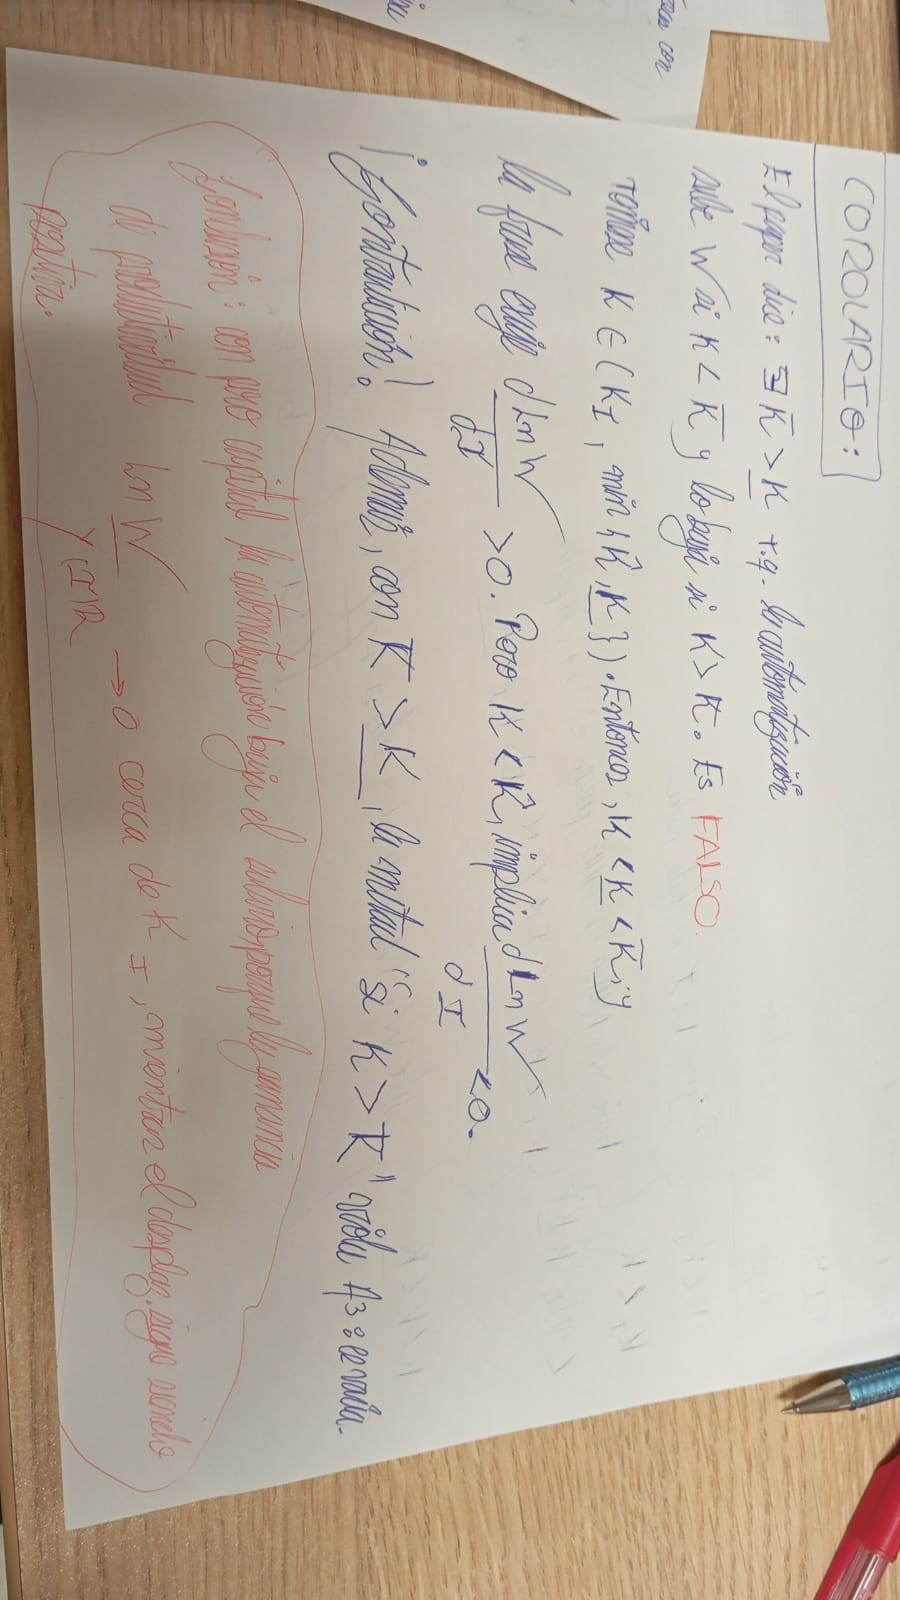
\includegraphics[angle=90,width=\linewidth,height=0.68\textheight,keepaspectratio]{hand/hand_6.jpeg}\\[-2pt]
{\tiny\texttt{hand/hand\_6.jpeg}: corolario, la frase impresa es falsa (derivación completa en \texttt{hand\_1}–\texttt{hand\_6})}
\end{columns}
\end{frame}

\begin{frame}{Lo que me parece poco convincente}
\begin{enumerate}\setlength\itemsep{3pt}
  \item \textbf{El umbral $\Kb$ de la Prop.~3}: dirección invertida, orden $\Kb>\Kl$ incompatible con el Supuesto~3, y el Apéndice~B no lo demuestra.
  \item \textbf{Homotecia de filo de navaja}: las fórmulas cerradas requieren $\eta\to0$ o $\zeta=1$; el caso general solo da resultados cualitativos.
  \item \textbf{$dN$ mezcla dos cosas}: la ventana $[N-1,N]$ tiene medida 1, así que una tarea nueva también \emph{elimina} una tarea automatizada. Parte de la ``reinstauración'' es mecánica.
  \item \textbf{El resultado de empleo} descansa en las preferencias de crecimiento balanceado (efecto ingreso).
  \item \textbf{El capital es igual de productivo en todas las tareas}, y la Figura~1 (títulos nuevos y empleo) es solo una correlación.
\end{enumerate}
\end{frame}

\begin{frame}{Extensión que puede crecer: la misma tecnología en economías con distinto capital}
Una tecnología de automatización común ($dI$) en dos economías con $K_S<K_N$ y ecuaciones (8)–(12) país por país:
\[
\frac{d\ln W_j}{dI}=\ln\frac{K_j}{K_{I,j}}-\frac{1}{(N-I)(1+\eps_{L,j})},\qquad j\in\{N,S\}.
\]
\begin{itemize}
  \item Si $K_S<\Kh_S$ y $K_N>\Kh_N$, el \emph{mismo} avance sube salarios en el Norte y los baja en el Sur.
  \item Con innovación dirigida a los precios del Norte: tecnología ``inapropiada'' para el Sur (en la línea de Acemoglu \& Zilibotti, 2001).
  \item Tres frentes: probar el cruce único con $\sh\neq1$; la dinámica (cuánto dura la caída mientras $K(t)<\Kh$); datos de capital por trabajador y robots (IFR) para el Perú.
  \item Revisado: los apéndices del paper no tienen versión de economía abierta.
\end{itemize}
\end{frame}

\begin{frame}[standout]
La automatización \emph{puede} subir el salario:\\ cuando el capital abunda lo suficiente, $K>\Kh$.\\[6pt]
\normalsize El paper imprime la dirección al revés; lo verificamos a mano, con 167\,639 checks y en Lean.\\[8pt]
\small\url{\repourl}
\end{frame}

\end{document}
